\documentclass{CLP}

%\usepackage{mathrsfs}

\begin{document}

\title{Title}

\author{Bajie Zhu (猪八戒)$^1$, and Daiyu Lin (林黛玉)$^{1^{*}}$}

\affil{MOE Key Laboratory of Material Physics and Chemistry under Extraordinary Conditions, and Shaanxi Key Laboratory of Optical Information Technology, School of Science, Northwestern Polytechnical University, Xi'an 710072, China}
\affil{Qian Xuesen laboratory of Space Technology, China Academy of Space Technology, Beijing 100094, China}

\corresp{\corsym{*}test@example.com}

\received{Month X, XXXX}
\accepted{Month X, XXXX}
\posted{Month X, XXXX}

\begin{abstract}
Abstract

\OCIScodes{keyword one, keyword two, keyword three.}

\doi{xxxxxxx/COLxxxxxxx.}
\end{abstract}
\maketitle

\section{This is first section with Level one head and is extended to second row}

% \subsection{This is First SubSection with Level TWO Head and is Extended to Second Row}
%
% \subsubsection{This is First SubSubSection with Level THREE Head and is Extended to Second Row}
%
% \paragraph{This is First ParaSection with Level FOUR Head and is Extended to Second Row}


\begin{figure}
\centering
	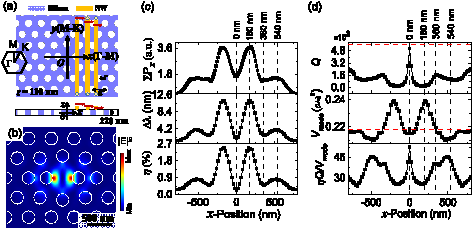
\includegraphics{Fig-example.pdf}
\caption{(a)citation}
\label{f1}
\end{figure}

\begin{table}
  \caption{Here is the Table caption extended to Second Row Second Row extended to Second Row}\label{tab1}
  {\tbodyfont\begin{tabular*}{\columnwidth}{@{\extracolsep{\fill}}lp{8pc}c@{}}
    \toprule
    \TCH{Head 1} & \TCH{Head 2} & \TCH{Head 3}\cr
    \colrule
    a & This is a para inside the table body & c \mycr
    d & e & f \mycr
    g & h & i \cr
    \botrule
  \end{tabular*}}
  {}
  \label{table1}
\end{table}


\begin{equation}
\begin{split}
\int_{-\infty}^{\infty} e^{-x^2} dx =& \lim_{a \to \infty} \int_{-a}^{a} e^{-x^2} dx
\end{split}
\label{eq1}
\end{equation}

test test Fig.\ref{f1} test test test Table.\ref{table1} test test test test test test test test test test Eq.\ref{eq1} test test test test test test test test test test test test test test test test test\cite{label1} test test test test test test test test test test test test test test test test test test test test test test 

test test Fig.\ref{f1} test test test Table.\ref{table1} test test test test test test test test test test Eq.\ref{eq1} test test test test test test test test test test test test test test test test test test test test test test test test test test test test test test test test test test test\cite{nat1} test test tes\cite{oe1} test 



% \begin{thebibliography}{26}
\bibliography{refs}
\bibliographystyle{col}
% \end{thebibliography}

\end{document}


